\cleardoublepage
\clearpage{}

%[Lo que va en el índice]{Lo que va en el documento}
\chapter[Implementación y experimentación]{Implementación y experimentación}

\section{KnowSeq}
Tras realizar las ejecuciones de \textit{KnowSeq} en los tres sistemas de archivos se obtuvieron los resultados que aparecen en el anexo \ref{resultados_knowseq}. Se han seguido las pautas especificadas en la metodología. \\

En primer lugar se creó la partición /dev/sda1 en el disco destinado a las pruebas. Acto seguido se creó y se montó el sistema de archivos. Tras esto el siguiente paso conseistía en  copiar los archivos necesarios para la ejecución de \textit{KnowSeq} en el disco y tras ello lanzar el script que automatiza la ejecución de la prueba y la recogida de datos a través de \textit{iowatcher}. Estos pasos se repitieron para cada uno de los tres sistemas de archivos.\\

La salida de \textit{iowatcher} consiste en una gráfica de la productividad en MB/s a través del tiempo y un archivo de texto con los ítems medidos, cuyo formato es poco amigable. La salida de \textit{iowatcher} para los tres sistemas es la que se muestran a continuación.\\ 

\begin{figure}[H]
    \centering
    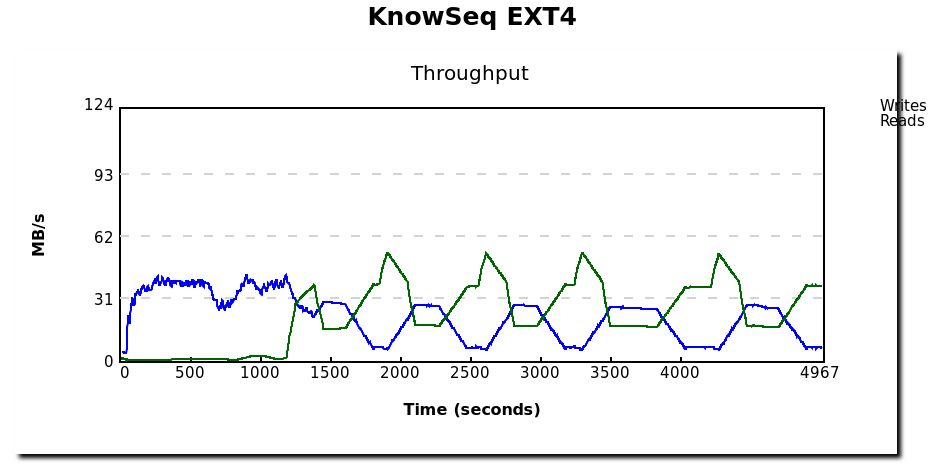
\includegraphics[scale=0.35]{doc/assets/images/Capitulo4/Knowseq/knowseq_ext4.png}
    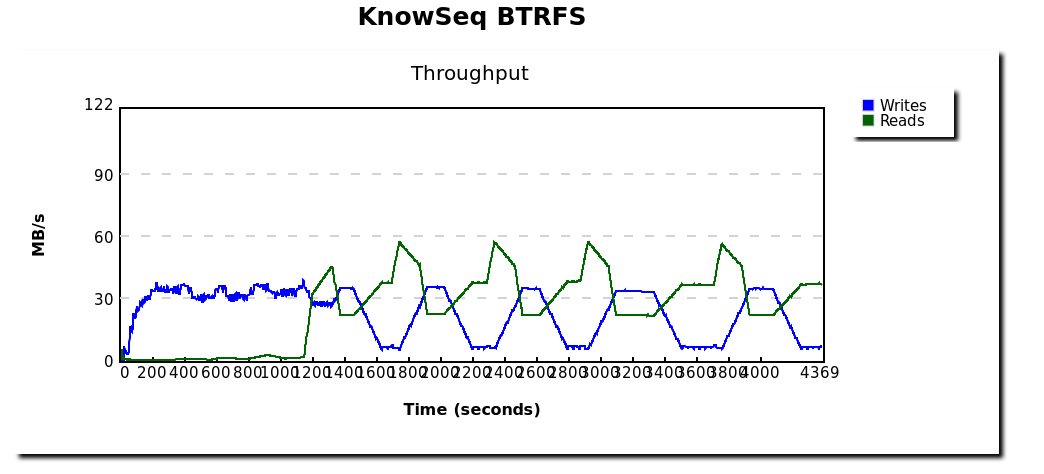
\includegraphics[scale=0.35]{doc/assets/images/Capitulo4/Knowseq/knowseq_btrfs.png}
    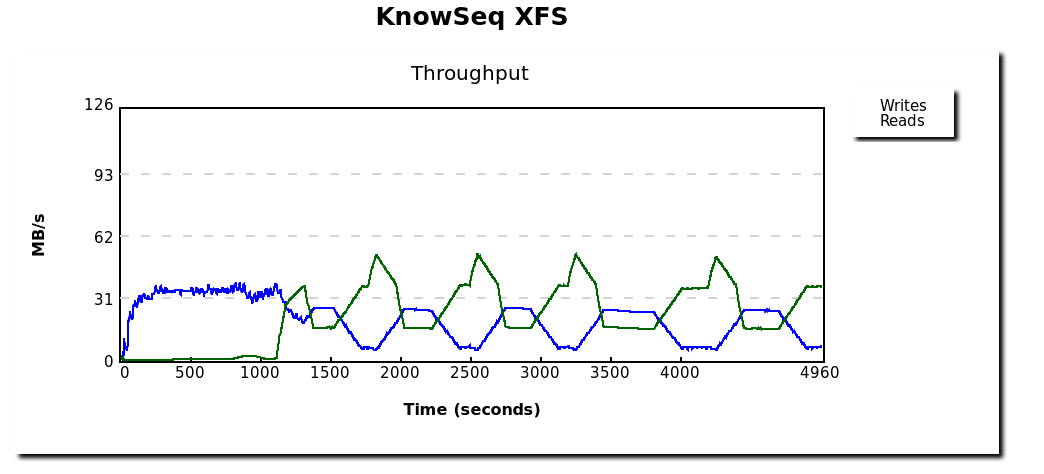
\includegraphics[scale=0.35]{doc/assets/images/Capitulo4/Knowseq/knowseq_xfs.png}
    \caption{Gráfica del rendimiento en \textit{KnowSeq} para cada sistema de archivos}
    \label{fig:my_label}
\end{figure}

Como se observa en las imágenes el patrón de velocidad de lecturas/escrituras es similar, esta situación puede ayudar a determinar que las pruebas han sido ejecutadas de forma correcta y que el programa en todos los casos realizó las mismas operaciones.

El siguiente paso consiste en transformar el archivo de texto que proporciona \textit{iowatcher} como salida ya que dicho documento no se encuentra en formato legible por el ser humano, para ello se utiliza \textit{blkparse}. La salida de \textit{blkparse}, entre otros muchos datos, nos proporciona la productividad en KiB/s. Con el fin de trabajar con unas unidades más usuales se decide transformar a MB/s y anotarlo en una hoja de cálculo y tras ello se calcula la media y desviación. Tal y como se puede ver en la tabla.

\begin{table}[H]\centering
\caption{Productividad de la prueba KnowSeq para EXT4, BTRFS y XFS}\label{tab: }
\scriptsize
\begin{tabular}{lrrrrrrr}\toprule
\textbf{Nº Ejecución} &\multicolumn{2}{c}{\textbf{EXT4}} &\multicolumn{2}{c}{\textbf{BTRFS}} &\multicolumn{2}{c}{\textbf{XFS}} \\\cmidrule{1-7}
&\textbf{Lectura} &\textbf{Escritura} &\textbf{Lectura} &\textbf{Escritura} &\textbf{Lectura} &\textbf{Escritura} \\\midrule
\textbf{1} &24.682 &21.703 &28.041 &24.574 &24.567 &21.533 \\
\textbf{2} &24.108 &21.143 &28.045 &24.568 &24.352 &21.402 \\
\textbf{3} &23.955 &20.977 &27.676 &24.258 &24.543 &21.570 \\
\textbf{4} &24.464 &21.498 &28.280 &24.795 &24.496 &21.529 \\
\textbf{} & & & & & & \\
\textbf{Promedio} &24.303 &21.330 &28.010 &24.549 &24.489 &21.508 \\
\textbf{Desviación} &0.331 &0.330 &0.250 &0.221 &0.096 &0.073 \\
\bottomrule
\end{tabular}
\end{table}
A partir de los datos de la tabla anterior podemos generar una gráfica con la media de la productividad.

\begin{figure}[H]
    \centering
    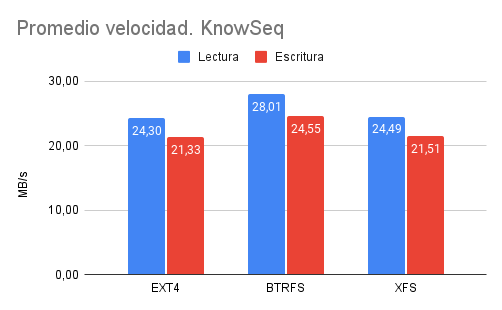
\includegraphics[scale=0.6]{doc/assets/images/Capitulo4/Knowseq/promknow.png}
    \caption{Productividad en MB/s de las pruebas usando KnowSeq y tres sistemas de archivos.}
    \label{aa}
\end{figure}

Se podría pensar que viendo la imagen \ref{aa} es suficiente para afirmar que BTRFS es mejor para el trabajo que realiza \textit{KnowSeq}. Pero surgen varias cuestiones ¿Es realmente mas productivo, o simplemente es casualidad o error en las mediciones?  ¿El utilizar un sistema de archivos u otro tiene que ver con la mejora de productividad?\\

Se decide por tanto realizar dos tests Anova del cual se habló en la sección \ref{anova_section}. Si tanto para lectura como para escritura se llega a la conclusión de que el factor sistema de archivos importa y es determinante.\\

Partimos de la hipótesis de que el rendimiento en lectura es igual para los tres sistemas de archivos y que el sistema de archivos no influye. Definimos la prueba al 95\% de confianza, es decir, $\alpha = 0.05$.\\

Generamos un csv con los datos en MB/s para cada sistema de archivos en lecturas y ejecutamos el script \ref{Anova.py} para el cálculo del \textit{p-value}. Obtenemos que el p-valor es $6.8424*10^{-9}$.\\

Para confirmar dicho resultado se repite el test con los mismos datos en la hoja de cálculo, cuyo resultado se refleja en la siguiente tabla. Se observa que obtenemos el mismo el p-valor. 

\begin{table}[!htp]\centering
\scriptsize
\begin{tabular}{lrrrrrrr}\toprule
Source of Variation &SS &df &MS &F &P-value &F crit \\\midrule
Between Groups &34.908 &2.0 &17.4541 &289.0014 &0.000000006842 &4.2565 \\
Within Groups &0.544 &9.0 &0.0604 & & & \\
& & & & & & \\
Total &35.452 &11.0 & & & & \\
\bottomrule
\end{tabular}
\caption{Resultado test Anova para las lecturas de \textit{KnowSeq}}\label{tab: }
\end{table}

Procedemos de la misma manera para realizar el test Anova para escritura con el objetivo de obtener un p-valor. Partimos de la hipótesis de que el rendimiento en escritura es igual en los tres sistemas de archivos. Ejecutamos el test Anova, y el resultado obtenido es el que se muestra en la siguiente tabla.

\begin{table}[!htp]\centering
\scriptsize
\begin{tabular}{lrrrrrrr}\toprule
Source of Variation &SS &df &MS &F &P-value &F crit \\\midrule
Between Groups &26.1819 &2 &13.0909 &240.5899 &0.00000001539899 &4.2565 \\
Within Groups &0.4897 &9 &0.0544 & & & \\
& & & & & & \\
Total &26.6716 &11 & & & & \\
\bottomrule
\end{tabular}
\caption{Resultado test Anova para las escrituras de \textit{KnowSeq}}\label{tab: }
\end{table}

Para finalizar se discutirán los resultados de los tests. Como en ambos test el \textit{p-value} es menor que $\alpha$ se rechazan ambas hipótesis nulas que se definieron al principio.\\

Se llega a la conclusión de que el rendimiento tanto en lectura como en escritura no es equivalente entre sistemas de ficheros. Es decir, existen diferencias significativas entre los sistemas de archivos para la ejecución de \textit{KnowSeq}. Por tanto se puede afirmar que BTRFS para la prueba KnowSeq es más productivo.

\section{Iozone}
Siguiendo las consideraciones que se detallaron en la sección \ref{metodologia_iozone} se ejecutaron los test. Desafortunadamente, debido al tiempo que tomaría y a la gran cantidad de datos que ello generaría se decidió repetir la prueba sólo cuatro veces, puesto que la desviación entre pruebas no es excesivamente alta. Es decir, se ha tenido que prescindir de la fórmula \ref{eqn:n-ejecuciones} para calcular el número de ejecuciones.\\

La salida de \textit{iozone} se presenta en formato tabla. La productividad depende por tanto del tamaño de archivo y del \textit{record size}. Con esta situación cabe preguntarse si las variaciones de dichos tamaños afectan realmente al rendimiento o no. Para ello se realiza un test Anova para comprobarlo.

\subsection{Test Anova para tamaño de archivo}
Para la realización de este test se realizaron 4 mediciones para tres configuraciones distintas de \textit{record size}. Por lo tanto se necesitan tres test, uno para cada tamaño de \textit{record size}.  Los resultados de dichas mediciones se pueden consultar en el Anexo \ref{tab:tabla_salida_anova_archivo}. Tras generar las tablas, se procede a ejecutar los test Anova. Antes se necesita especificar cual es la hipótesis nula, en este caso, la hipótesis es que el rendimiento es  igual para cualquier tamaño de archivo. La salida obtenida es la siguiente. 

\begin{table}[H]\centering
\scriptsize
\begin{tabular}{lrrrrrrr}\toprule
Source of Variation &SS &df &MS &F &P-value &F crit \\\midrule
Between Groups &16353394702915.422 &13 &1257953438685.8018 &89.29416792 &0 &1.9612184003 \\
Within Groups &591685276360.5 &42 &14087744675.25 & & & \\
& & & & & & \\
Total &16945079979275.922 &55 & & & & \\
\bottomrule
\end{tabular}
\caption{Resultado test Anova para comprobar si el tamaño de archivo es un factor que afecta a la productividad con un tamaño de \textit{record size de 64KB}}\label{tab: }
\end{table}

\begin{table}[H]\centering
\scriptsize
\begin{tabular}{lrrrrrrr}\toprule
Source of Variation &SS &df &MS &F &P-value &F crit \\\midrule
Between Groups &13060330768231.422 &13 &1004640828325.494 &61.457186809122 &0 &1.96121840 \\
Within Groups &686574133644 &42 &16347003182 & & & \\
& & & & & & \\
Total &13746904901875.422 &55 & & & & \\
\bottomrule
\end{tabular}
\caption{Resultado test Anova para comprobar si el tamaño de archivo es un factor que afecta a la productividad con un tamaño de \textit{record size de 1024KB}}\label{tab: }
\end{table}

\begin{table}[H]\centering
\scriptsize
\begin{tabular}{lrrrrrrr}\toprule
Source of Variation &SS &df &MS &F &P-value &F crit \\\midrule
Between Groups &12138841872010.5 &9 &1348760208001.1667 &173.4900496764 &0 &2.21069698 \\
Within Groups &233228397337.5 &30 &7774279911.25 & & & \\
& & & & & & \\
Total &12372070269348 &39 & & & & \\
\bottomrule
\end{tabular}
\caption{Resultado test Anova para comprobar si el tamaño de archivo es un factor que afecta a la productividad con un tamaño de \textit{record size de 16384KB}}\label{tab: }
\end{table}

Como para los tres tamaños de \textit{record size} $p-value < 0.05$ se rechaza la hipótesis planteada. El tamaño de archivo \textbf{si} es un factor que influye en la productividad.

\subsection{Test Anova para \textit{record size}}
De igual manera se procede en este caso. Fijamos tres tamaños de archivos, en este caso 512MB, 2GB y 8GB. Los tamaños de record size van a ser los que varíen. Igual que en el test anterior se ha repetido la prueba 4 veces para cada tamaño de archivo. La hipótesis nula es que el \textit{record size} no es un factor que influya en el rendimiento. Los resultados para los tres test son los siguientes:

\begin{table}[H]\centering
\scriptsize
\begin{tabular}{lrrrrrrr}\toprule
Source of Variation &SS &df &MS &F &P-value &F crit \\\midrule
Between Groups &7157416779626.656 &11 &650674252693.3324 &188.781965827 &0 &2.066608478 \\
Within Groups &124081095322 &36 &3446697092.2777777 & & & \\
& & & & & & \\
Total &7281497874948.656 &47 & & & & \\
\bottomrule
\end{tabular}
\caption{Resultado test Anova para comprobar si el tamaño de \textit{record size} es un factor que afecta a la productividad con un tamaño de archivo de 512MB}\label{tab: }
\end{table}

\begin{table}[H]\centering

\scriptsize
\begin{tabular}{lrrrrrrr}\toprule
Source of Variation &SS &df &MS &F &P-value &F crit \\\midrule
Between Groups &653116815773.2305 &11 &59374255979.38459 &5.2127172 &0.00007428 &2.0666084 \\
Within Groups &410049713763.25 &36 &11390269826.756945 & & & \\
& & & & & & \\
Total &1063166529536.4805 &47 & & & & \\
\bottomrule
\end{tabular}
\caption{Resultado test Anova para comprobar si el tamaño de \textit{record size} es un factor que afecta a la productividad con un tamaño de archivo de 2GB}\label{tab: }
\end{table}

\begin{table}[!htp]\centering

\scriptsize
\begin{tabular}{lrrrrrrr}\toprule
Source of Variation &SS &df &MS &F &P-value &F crit \\\midrule
Between Groups &541800093953.917 &11 &49254553995.81064 &27.175544410 &3.619327e-14 &2.06660847825 \\
Within Groups &65248515984 &36 &1812458777.33333 & & & \\
& & & & & & \\
Total &607048609937.917 &47 & & & & \\
\bottomrule
\end{tabular}
\caption{Resultado test Anova para comprobar si el tamaño de \textit{record size} es un factor que afecta a la productividad con un tamaño de archivo de 8GB}\label{tab: }
\end{table}


Los p-valores en los tres casos son menores que el grado de significatividad $\alpha = 0,05$ por lo que en los tres casos rechazamos la hipótesis nula. El tamaño de \textit{record size} afecta a la productividad.

\subsection{Test Anova para Sistema de Archivos}
Para la realización de los test siguientes se han seguido las siguientes pautas.
\begin{itemize}
    \item Cuatro repeticiones por tamaño de \textit{record length}.
    \item Se realiza la prueba para seis operaciones (read/re-read, write/re-write, random-read/random-write).
    \item Tamaños de archivo de 200MB, 400MB, 800MB, 1.6GB, 3.2GB y 6GB.
    \item Tamaños para \textit{record length} de 4KB, 256KB, 1024KB y 16384KB
\end{itemize}

El objetivo es analizar si para una operación, tamaño de archivo y \textit{record length} concreto el factor sistema de archivos afecta al rendimiento. Por lo que se tendrán que realizar test Anova correspondientes fijando ambos tamaños por cada operación. Las salidas de iozone para cada test se encuentran en el anexo 